\documentclass{article}
\usepackage{ctex}
\usepackage{graphicx}
\usepackage{amsmath}
\usepackage{indentfirst}
\usepackage{titlesec}
\usepackage{setspace}
\usepackage{subfigure}
\usepackage{caption}
\usepackage{float}
\usepackage{booktabs}
\usepackage{geometry}
\usepackage{multirow}
\usepackage{hyperref}
\hypersetup{
	colorlinks=true,
	linkcolor=blue,
	filecolor=magenta,      
	urlcolor=cyan,
	pdftitle={Overleaf Example},
	pdfpagemode=FullScreen,
}
\geometry{left=1.2cm,right=1.2cm,top=2cm,bottom=2cm}
\title{\songti \zihao{2}\bfseries HW7第12题逾渗}
\titleformat*{\section}{\songti\zihao{4}\bfseries}
\titleformat*{\subsection}{\songti\zihao{5}\bfseries}
\renewcommand\thesection{\arabic{section}}
\author{王启骅 PB20020580}
\begin{document}
	\maketitle
	\section{题目}
	推导正方格子点阵上键逾渗的重整化群变换表达式 p’ = R(p),求临界点 $ p_c $
	与临
	界指数 $ \nu $,与正确值(表1.6.1.3-1)相比较。
	
	\section{算法原理}
	对于正方形点阵键渝渗的重整化的思路如下图\ref{fig:1}
	\begin{figure}[!h]
		\centering
		\subfigure[重整化对象]{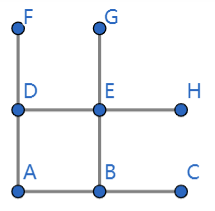
\includegraphics[scale=1.5]{Bond_8}}
		\subfigure[原胞]{	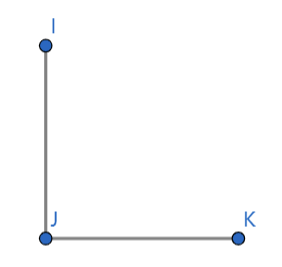
\includegraphics[scale=1]{bond_2}}
		\captionsetup{font={small},labelfont=bf}
		\caption{\heiti\zihao{-5}正方形点阵键渝渗的重整化}
		\label{fig:1}
	\end{figure}
我们将如图\ref{fig:1}(a)所示的键结构重整化为(b)所示的原胞。我们可以通过水平、竖直方向的平移验证得到 (a)的确可以作为一个重整化的元。


接下来我们考虑可以竖直连通的情况,共有一下情况
	\begin{figure}[!h]
	
	\centering
	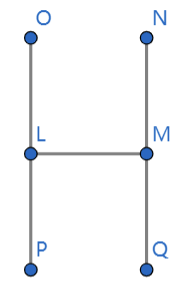
\includegraphics[scale=0.5]{bond_5}
	\captionsetup{font={small},labelfont=bf}
	\caption{\heiti\zihao{-5}5键连通}
	\label{fig:2}
\end{figure}
	
	\begin{figure}[!h]
	\centering
	\subfigure[组合1]{\includegraphics[scale=0.5]{Bond_4}}
	\subfigure[组合2]{	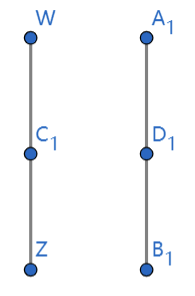
\includegraphics[scale=0.5]{bond_41}}
	\captionsetup{font={small},labelfont=bf}
	\caption{\heiti\zihao{-5}4键连通}
	\label{fig:3}
\end{figure}
	\begin{figure}[!h]
	\centering
	\subfigure[组合1]{\includegraphics[scale=0.5]{Bond_3}}
	\subfigure[组合2]{	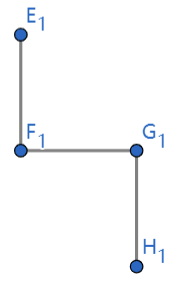
\includegraphics[scale=0.5]{bond_31}}
	\captionsetup{font={small},labelfont=bf}
	\caption{\heiti\zihao{-5}3键连通}
	\label{fig:4}
\end{figure}
	\begin{figure}[!h]
	
	\centering
	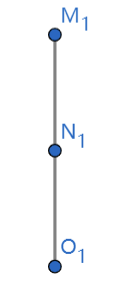
\includegraphics[scale=0.5]{bond_21}
	\captionsetup{font={small},labelfont=bf}
	\caption{\heiti\zihao{-5}2键连通}
	\label{fig:5}
\end{figure}
对以下情况计数分析可以得到图\ref{fig:2}存在1种情况,对应概率$ p^5 $。图\ref{fig:3}(a)存在4种情况,(b)存在1种情况,对应概率$ 5p^4(1-p) $。图\ref{fig:4}(a)存在6种情况,(b)存在2种情况,对应概率$ 8p^3(1-p)^2 $。最后图\ref{fig:5}存在一种情况,概率$ p^2(1-p)^3 $。于是得到
\begin{equation}
	\begin{aligned}
		R(p)&=p^5+5p^4(1-p)+8p^3(1-p)^2+2p^2(1-p)^3\\
		&=2p^5-5p^4+2p^3+2p^2
	\end{aligned}
\end{equation}


求取不动点
\begin{equation}
	p=2p^5-5p^4+2p^3+2p^2
\end{equation}
解得$ p*=0,\ 1,\ 0.5,\ -0.618034,\ 1.61803 $,则有(0,1)间的非平凡解$ p_c=0.5 $


这里由于原胞的边长变化缩小了2倍,有b=2 。根据关联长度$ \xi'=\xi/b $,在$ p\sim p_c $处有$ \xi(p)\propto |p-p_c|^{-\nu} $,故得
\begin{equation}
	|p'-p^*|^{-\nu}=b^{-1}|p-p^*|^{-\nu}
	\label{eq3}
\end{equation}
取Taylor展开1级近似
\begin{equation}
	p'-p^*=R(p)-R(p^*)=\dfrac{R}{p}(p^*)(p-p^*)
	\label{eq4}
\end{equation}
\begin{equation}
	\dfrac{dR}{dp}(p^*)=10p^4-20p^3+6p^2+4p=\frac{13}{8}
\end{equation}
将(\ref{eq3}),(\ref{eq4})联立可得
\begin{equation}
	\nu=\frac{\ln(b)}{\ln(\dfrac{dR}{dp}(p^*))}=1.428
\end{equation}


与讲义中表格对比可得,计算得到临界点 $ p_c=0.5 $与讲义中正确值完全相等,而临界指数计算值$ \nu=1.428 $与正确值4/3也较为接近。
	\section{结论}
	根据计算结果,计算得到的临界点$ p_c $与正确值完全相符,说明该正方形键逾渗的模型取如此的基元进行重整化具有较为特殊的对称性与自相似性,可以良好的近似得到真是结果。
	
	
	但是对于临界指数的计算仍然与真实值具有一定的偏差,可能是由于所取的基元尺寸较小,键格较少,从而受到边界效应的影响,重整化后导致原始的态受到破坏。如果取b较大,则可以更加接近真实值,减小误差。
\end{document}